\documentclass[11pt]{article}

\usepackage[margin=1in]{geometry}
\usepackage{amsmath}
\usepackage{booktabs}
\usepackage{graphicx}
\usepackage{microtype}
\usepackage{tabularx}
\usepackage[numbers,sort&compress]{natbib}
\usepackage{xcolor}
\usepackage[hidelinks]{hyperref}
\usepackage{url}
\usepackage[UTF8,fontset=fandol]{ctex}
\setlength{\emergencystretch}{1em}

\newcommand{\method}{匹配的位置--监督析因研究}
\newcommand{\pending}[1]{\textcolor{red}{[待定：#1]}}
% Generated from audited seed-level result JSON; do not hand-edit.
\newcommand{\ExploratoryRuleAnswerMin}{97.3\%}
\newcommand{\ExploratoryRuleAnswerMax}{100.0\%}
\newcommand{\ExploratoryPairedAnswerWorst}{87.3\%}
\newcommand{\ExploratoryPairedAnswerGap}{12.7\%}
\newcommand{\ExploratoryIndependentEvidenceWorst}{99.7\%}
\newcommand{\ExploratoryIndependentEvidenceGap}{0.3\%}
\newcommand{\GeneratedMainRows}{%
Mistral-7B-v0.3 & -- & -- & 63.3 & 39.0 & 60.7 & 53.4 \\
Mistral-7B-v0.3 & Independent & Answer & 95.4 & 89.9 & 10.1 & 0.0 \\
Mistral-7B-v0.3 & Independent & Evidence ID & 92.5 & 84.2 & 15.6 & 0.0 \\
Mistral-7B-v0.3 & Independent & Exact evidence & 77.1 & 69.6 & 17.9 & 76.7 \\
Mistral-7B-v0.3 & Paired & Answer & 75.8 & 63.7 & 26.1 & 0.0 \\
Mistral-7B-v0.3 & Paired & Evidence ID & 94.4 & 88.5 & 11.5 & 0.0 \\
Mistral-7B-v0.3 & Paired & Exact evidence & 99.4 & 96.7 & 3.3 & 82.9 \\
\addlinespace
Qwen2.5-7B & -- & -- & 69.2 & 41.5 & 51.2 & 68.3 \\
Qwen2.5-7B & Independent & Answer & 98.0 & 92.9 & 7.1 & 0.0 \\
Qwen2.5-7B & Independent & Evidence ID & 99.7 & 98.7 & 1.3 & 0.0 \\
Qwen2.5-7B & Independent & Exact evidence & 99.6 & 97.9 & 2.1 & 99.8 \\
Qwen2.5-7B & Paired & Answer & 97.2 & 90.8 & 9.2 & 0.0 \\
Qwen2.5-7B & Paired & Evidence ID & 99.7 & 98.2 & 1.8 & 0.0 \\
Qwen2.5-7B & Paired & Exact evidence & 99.5 & 97.6 & 2.4 & 99.8 \\
}
\newcommand{\GeneratedNoLiMaRows}{%
Mistral-7B-v0.3 & -- & -- & 12.9 & 4.8 & 32.6 & 16.7 \\
Mistral-7B-v0.3 & Independent & Answer & 9.8 & 2.3 & 32.1 & 0.0 \\
Mistral-7B-v0.3 & Independent & Evidence ID & 18.4 & 7.4 & 34.8 & 0.0 \\
Mistral-7B-v0.3 & Independent & Exact evidence & 16.7 & 4.0 & 50.6 & 10.5 \\
Mistral-7B-v0.3 & Paired & Answer & 4.0 & 0.0 & 21.0 & 0.0 \\
Mistral-7B-v0.3 & Paired & Evidence ID & 17.9 & 7.8 & 35.7 & 0.0 \\
Mistral-7B-v0.3 & Paired & Exact evidence & 13.8 & 4.6 & 34.1 & 16.2 \\
\addlinespace
Qwen2.5-7B & -- & -- & 17.7 & 7.0 & 40.4 & 13.8 \\
Qwen2.5-7B & Independent & Answer & 13.0 & 1.7 & 40.4 & 0.0 \\
Qwen2.5-7B & Independent & Evidence ID & 13.3 & 2.6 & 36.2 & 0.0 \\
Qwen2.5-7B & Independent & Exact evidence & 15.5 & 3.2 & 44.2 & 11.0 \\
Qwen2.5-7B & Paired & Answer & 15.7 & 2.3 & 51.9 & 0.0 \\
Qwen2.5-7B & Paired & Evidence ID & 13.7 & 3.8 & 37.2 & 0.0 \\
Qwen2.5-7B & Paired & Exact evidence & 15.5 & 5.6 & 42.2 & 13.9 \\
}
\newcommand{\GeneratedLongBenchRows}{%
Mistral-7B-v0.3 & -- & -- & 46.4 & 28.3 & 23.4 & 32.7 \\
Mistral-7B-v0.3 & Independent & Answer & 47.8 & 31.0 & 20.6 & 33.1 \\
Mistral-7B-v0.3 & Independent & Evidence ID & 52.1 & 37.9 & 24.8 & 38.3 \\
Mistral-7B-v0.3 & Independent & Exact evidence & 29.7 & 23.3 & 14.9 & 22.6 \\
Mistral-7B-v0.3 & Paired & Answer & 35.6 & 25.0 & 15.1 & 25.2 \\
Mistral-7B-v0.3 & Paired & Evidence ID & 50.8 & 36.3 & 22.4 & 36.5 \\
Mistral-7B-v0.3 & Paired & Exact evidence & 27.4 & 24.7 & 14.3 & 22.1 \\
\addlinespace
Qwen2.5-7B & -- & -- & 58.3 & 43.3 & 29.5 & 43.7 \\
Qwen2.5-7B & Independent & Answer & 53.2 & 44.3 & 23.1 & 40.2 \\
Qwen2.5-7B & Independent & Evidence ID & 52.0 & 42.2 & 22.6 & 39.0 \\
Qwen2.5-7B & Independent & Exact evidence & 55.8 & 44.7 & 27.5 & 42.7 \\
Qwen2.5-7B & Paired & Answer & 55.5 & 45.7 & 27.1 & 42.8 \\
Qwen2.5-7B & Paired & Evidence ID & 55.2 & 42.2 & 26.5 & 41.3 \\
Qwen2.5-7B & Paired & Exact evidence & 55.5 & 43.4 & 28.0 & 42.3 \\
}
\newcommand{\GeneratedFactorialContrastRows}{%
Mistral-7B-v0.3 & Paired $-$ independent & +1.7 [-78.7, +82.2] & -0.9 [-55.6, +53.8] & -0.5 [-5.4, +4.5] & -8.9 [-27.3, +9.4] & -3.4 [-17.8, +11.1] \\
Mistral-7B-v0.3 & Evidence ID $-$ answer & +9.6 [-32.3, +51.5] & -4.5 [-27.4, +18.3] & +6.4 [+0.9, +12.0] & +8.7 [-4.7, +22.1] & +8.2 [-10.1, +26.6] \\
Mistral-7B-v0.3 & Exact evidence $-$ answer & +6.4 [-66.2, +78.9] & -7.5 [-42.7, +27.8] & +3.1 [-2.9, +9.1] & +15.8 [-9.1, +40.7] & -6.8 [-15.5, +2.0] \\
Mistral-7B-v0.3 & Pairing $\times$ exact-vs-answer & +53.3 [+8.7, +97.9] & -30.6 [-35.4, -25.8] & +3.0 [-1.6, +7.6] & -5.4 [-58.6, +47.7] & +7.4 [-34.0, +48.7] \\
\addlinespace
Qwen2.5-7B & Paired $-$ independent & -1.0 [-5.4, +3.4] & +1.0 [-3.4, +5.4] & +1.4 [-1.7, +4.5] & +3.5 [-16.4, +23.4] & +1.5 [-2.5, +5.5] \\
Qwen2.5-7B & Evidence ID $-$ answer & +6.5 [-6.5, +19.6] & -6.5 [-19.6, +6.5] & +1.2 [+0.5, +1.9] & -9.4 [-17.9, -1.0] & -1.4 [-7.9, +5.2] \\
Qwen2.5-7B & Exact evidence $-$ answer & +5.9 [-6.5, +18.3] & -5.9 [-18.3, +6.5] & +2.3 [+1.6, +3.0] & -2.9 [-27.2, +21.4] & +1.0 [+0.2, +1.8] \\
Qwen2.5-7B & Pairing $\times$ exact-vs-answer & +1.8 [-3.4, +7.0] & -1.8 [-7.0, +3.4] & +1.7 [-2.6, +6.1] & -13.5 [-54.7, +27.7] & -3.0 [-10.1, +4.1] \\
}
\newcommand{\GeneratedRegressionRows}{%
Qwen2.5-7B & -- & -- & 67.0 & -- & 72.5 & -- \\
Qwen2.5-7B & Independent & Answer & 66.7 & Pass & 70.2 & Fail \\
Qwen2.5-7B & Independent & Evidence ID & 66.6 & Pass & 69.5 & Fail \\
Qwen2.5-7B & Independent & Exact evidence & 67.0 & Pass & 71.5 & Fail \\
Qwen2.5-7B & Paired & Answer & 66.8 & Pass & 69.7 & Fail \\
Qwen2.5-7B & Paired & Evidence ID & 66.3 & Pass & 70.4 & Fail \\
Qwen2.5-7B & Paired & Exact evidence & 66.4 & Pass & 71.3 & Fail \\
\addlinespace
Mistral-7B-v0.3 & -- & -- & 54.2 & -- & 43.1 & -- \\
Mistral-7B-v0.3 & Independent & Answer & 52.6 & Fail & 40.1 & Fail \\
Mistral-7B-v0.3 & Independent & Evidence ID & 54.9 & Pass & 42.9 & Fail \\
Mistral-7B-v0.3 & Independent & Exact evidence & 53.6 & Pass & 45.1 & Pass \\
Mistral-7B-v0.3 & Paired & Answer & 34.3 & Fail & 21.3 & Fail \\
Mistral-7B-v0.3 & Paired & Evidence ID & 53.2 & Pass & 39.2 & Fail \\
Mistral-7B-v0.3 & Paired & Exact evidence & 53.8 & Pass & 40.7 & Fail \\
}
\newcommand{\GeneratedMechanismRows}{%
Qwen2.5-7B & -- & -- & 17.7 & 6.0 & 0.7 & 100.0 \\
Qwen2.5-7B & Independent & Answer & 10.8 & 0.0 & 0.7 & 98.0 \\
Qwen2.5-7B & Independent & Exact evidence & 18.2 & 34.7 & 5.3 & 100.0 \\
Qwen2.5-7B & Paired & Answer & 16.1 & 0.0 & 2.0 & 100.0 \\
Qwen2.5-7B & Paired & Exact evidence & 15.6 & 35.8 & 0.7 & 99.3 \\
\addlinespace
Mistral-7B-v0.3 & -- & -- & 12.9 & 34.8 & 54.7 & 100.0 \\
Mistral-7B-v0.3 & Independent & Answer & 14.3 & 0.0 & 96.7 & 72.7 \\
Mistral-7B-v0.3 & Independent & Exact evidence & 24.2 & 6.2 & 84.7 & 98.7 \\
Mistral-7B-v0.3 & Paired & Answer & 0.2 & 0.0 & 10.0 & 88.0 \\
Mistral-7B-v0.3 & Paired & Exact evidence & 16.8 & 13.9 & 84.0 & 89.3 \\
}


\title{配对位置，还是监督证据？\\
长上下文位置稳健性的匹配析因研究}
\author{\pending{作者姓名、排序、单位与联系邮箱}}
\date{}

\begin{document}
\maketitle

\begin{abstract}
长上下文语言模型在相关证据于输入内移动、其余内容不变时，回答可靠性往往下降。既有训练研究同时改变多个因素，因此无法区分改进究竟来自重复事实、均衡位置、显式跨位置配对，还是更丰富的证据监督。我们提出一项算力匹配的 $2\times3$ 析因研究，独立地变化位置构造（独立采样对配对）与监督粒度（仅答案、证据 ID、精确证据引文）。每一严格对比都固定事实、曝光计数、填充文档实现、序列数、位置直方图与输入 token 预算。我们在七位置受控测试上评测答案正确性、证据可验证性、最差位置准确率与位置差距；在 NoLiMa 上评测无字面重叠的语义检索；在 LongBench 上评测自然多文档迁移。每个模型家族使用三个固定训练/数据种子，并披露一项实际采样器审计：该审计将最初不完整的 Qwen 配对实现降级为探索性结论，随后以块完备适配器重跑。在 Qwen2.5-7B 与 Mistral-7B 两个家族上，单次 96 步训练将受控测试的最差位置准确率从 41.5/39.0（各家族基座）修复到 63.7--98.7，但起修复作用的因素随家族而异：Qwen 上监督粒度区分各单元，而 Mistral 呈现 $+53.3$ 个百分点 $[+8.7,+97.9]$ 的配对$\times$监督交互。在 NoLiMa 上没有任何处理稳定超过其未训练基座（Qwen 各单元 13.0--15.7，基座 17.7；仅 Mistral 的证据 ID 单元为 17.9--18.4，基座 12.9），自然 LongBench 迁移上监督粒度效应在两家族间反号（Mistral 证据 ID $+5.6$、精确引文 $-10.1$ 个百分点对基座；Qwen 为 $-0.9$ 至 $-4.7$）。我们的结果区分了分布特定修复与稳健的长上下文利用，并提供一套可审计的协议，用于把增益归因于训练位置结构与监督内容。
\end{abstract}

\section{引言}

支持长输入并不等于可靠地使用其中每一部分。位置受控评测表明，移动同一段相关文本即可改变模型行为，在上下文边界处常强于中部 \citep{liu2024lost}。该曲线并非普适：其形状取决于相对输入长度、任务结构与检索难度。此外，字面针测试可能高估可用上下文，因为模型可以利用词法匹配，而非恢复潜在关联 \citep{modarressi2025nolima}。

以信息密集、乱序或证据接地的长上下文样本训练可以压平位置曲线 \citep{an2024film,he2024never,yuan2026longcrafter}。然而既有干预通常同时改变数据量、任务多样性、难度、证据格式与位置分布。因此，改进无法被干净地归因于：在更多位置看到事实、在跨位置看到\emph{同一}事实，还是获得了显式指认支持证据的目标。

我们用匹配析因设计分离这些因素。位置因素对比独立位置采样与显式位置等价配对；监督因素对比仅答案目标、答案加证据文档 ID、答案加精确原文引文。六个单元在匹配的序列与 token 预算下使用相同事实与填充视图。该设计提出两个聚焦问题：(i) 显式跨位置配对能否在位置均衡的独立采样之上改善最弱位置；(ii) 逐步可验证的监督改变的是答案稳健性，还是仅输出格式。

我们的贡献为：
\begin{itemize}
    \item 针对位置构造与监督粒度的匹配 $2\times3$ 因果归因设计；
    \item 位置等价评测协议，报告最差位置准确率、差距、证据有效性与配对不确定性，而非仅平均准确率；
    \item 互补的分布偏移测试：受控 NoLiMa 语义检索与自然 LongBench 多文档问答（QA）；
    \item 可复现性包，包含数据生成审计、模型与环境哈希、逐步训练轨迹、许可安全的逐样本审计记录与保存的自助法索引。
\end{itemize}

\section{相关工作}

\paragraph{位置相关的上下文利用。}
Lost in the Middle 建立了受控多文档 QA 与键--值检索测试：相关内容位置改变而内容不变 \citep{liu2024lost}。RULER 基准套件将合成长上下文评测拓宽到检索、追踪、聚合与问答 \citep{hsieh2024ruler}。LongBench 以 21 个自然与合成任务补充受控测试，但其本身无法识别因果位置效应 \citep{bai2024longbench}。NoLiMa 去除问题与证据间的直接词法匹配，显示许多模型在宣传的上下文上限之前就已退化 \citep{modarressi2025nolima}。Veseli 等人按各模型最大上下文归一化输入长度，指出熟悉的 U 形在相对长度不超过一半时最强；接近上限时首因减弱而近因保留，因此缺少 U 形并不必然意味着位置不变 \citep{veseli2025shift}。CRE 通过在 GSM8K 与 AI2 Reasoning Challenge (ARC)-Challenge 上联合变化目标位置、填充内容与上下文长度，独立审计推理基准差距；其依赖模型与填充的失败强化了报告位置条件化而非聚合分数的必要性 \citep{zhang2026positional}。我们将严格的组内位置控制与自然迁移结合，而不将任一方视为单独充分。

这些评测研究确立了现象，但未指明哪种训练数据属性可以修复它。特别地，CRE 改变评测上下文而保持被测模型固定，Veseli 等人刻画跨相对长度的曲线形状。我们的贡献与之正交：在身份、曝光、序列与提示 token 匹配的预算下随机化训练位置构造与目标监督，再检验任何由此产生的修复能否迁移到它们更难的语义与自然场景。因此我们不声称受控基准或位置度量本身是新的。

一项并行的的小型 Transformer 研究给出了互补的可识别性警告：当位置与重复线索在合成文档分布中恰好共变时，所有运行都能达到近乎完美的留内准确率，而基于干预的规则读出在不同种子间剧烈变化 \citep{liao2026shortcut}。该研究关注合成预训练期间的机制选择而非长上下文适配，因此不是我们 7B 模型的干预基线。但它促使我们分离共变的训练因素，并将独立训练种子作为复现单元，而非仅从聚合准确率推断机制。

\paragraph{推理时与位置编码干预。}
Found in the Middle 通过移动固定上下文估计一个与内容无关的位置注意力基线，随后为检索增强生成（RAG）校准文档注意力；它改进了 NaturalQuestions 与 SynthWiki，但对 $K$ 个文档位置需要额外 $O(K)$ 次前向 \citep{hsieh2024found}。LPES 方法则在 200 个样本上搜索平滑的逐层 RoPE 缩放曲线，不改动模型权重，搜索后单次前向 \citep{lv2026lpes}。二者都作用于推理或位置编码。本研究提出的是不同的训练时归因问题：在固定事实、曝光、序列与提示 token 预算下，保持身份的跨位置配对或更丰富的监督目标能否产生可迁移的稳健性？因此我们不声称这些方法可互换，并将架构或推理时组合留给未来工作。

\paragraph{训练干预。}
Position-Agnostic Multi-step QA 在乱序文档上训练问题重复、证据索引预测与答案生成 \citep{he2024never}。IN2 构造关键片段分布贯穿长上下文的信息密集样本 \citep{an2024film}。LongCrafter 用任务分类法、证据约束图与带引用的回答生成困难且忠实的长上下文监督 \citep{yuan2026longcrafter}。这些研究确立了数据设计的重要性，但未在等预算下完全分离显式跨位置配对与目标的信息内容。我们的证据 ID 单元是仅答案与精确引文之间的中间处理，允许对定位监督做分级检验。

Pos2Distill 是最接近的同样本跨位置先例：检索变体将优势证据位置处的输出分布以 Kullback--Leibler (KL) 目标迁移到劣势位置，推理变体跨位置蒸馏高质量思维链 \citep{wang2025pos2distill}。它因此同时引入位置配对、非对称教师--学生方向与专门化蒸馏目标。本研究不声称跨位置身份复用是新的；其析因控制检验的是：保持身份的配对本身是否在匹配的独立位置直方图之上有贡献，以及任何效应是否依赖于答案、证据 ID 或精确引文监督——在无教师模型、无 KL 损失的前提下。

RoPE 扰动自蒸馏对同一长序列构造标准与索引平移两个视图，加入 stop-gradient 反向 KL 一致性损失；它在 RULER 与 HELMET 基准套件上报告双家族增益、长度外推、LongBench-v2 迁移、短任务保持与匹配墙时对照 \citep{li2026shuffle}。随机化 YaRN 则在短上下文 LoRA 中按扩张课程分配有序随机 YaRN 索引，并在两个 7B 家族上于 BABILong 与 MRCR 评测超越训练长度的推理 \citep{mehta2026randomized}。这些是重要的正向干预基线，但二者都改变了位置编码暴露与优化目标。我们固定 RoPE、推理与仅完成部分优化，以隔离数据身份配对与监督内容；因此我们的阴性或零迁移结果不与更强位置编码正则化的增益相矛盾。

FOCUSFT 处理另一种训练机制：内层快权重回路形成上下文条件化的参数记忆，外层监督微调（SFT）回路从该锐化表示学习，两回路均对上下文 token 使用双向注意力 \citep{pei2026focusft}。它以不变推理成本报告强 BABILong 与 RULER 增益，但仅用一个 Qwen2.5-7B 家族且训练墙时增加 1.71 倍。我们固定的仅完成 QLoRA 目标保持注意力掩码与优化结构不变，使本研究问题更窄：哪些匹配的数据构造与目标内容（若有）能改进稳健性？

EXACT 方法分离了一个互补的目标层干预：在打包的继续预训练流、token 预算、优化器与后续 QA 微调固定的条件下，对同文档有效左上下文较长的稀有目标加权 \citep{zhu2026exact}。其对照区分了有效上下文加权与随机加权及绝对打包位置加权，但未比较同一底层事实是否被显式跨位置配对，也未比较答案、标识符与精确引文目标在匹配的仅完成 SFT 下的差异。因此我们的析因分析回答的是数据身份与目标内容问题，而非因果语言模型损失分配问题。

纵观评测、推理时与训练干预，尚无研究在固定事实、曝光、填充实现、序列数、位置直方图与提示 token 预算的同时分别变化位置构造与监督粒度，也没有报告此类增益能否迁移到无字面重叠的语义检索。这一归因缺口正是本研究的对象。

\section{实验设计}

\subsection{匹配析因处理}

设 $f$ 为底层事实集，$v$ 为固定填充实现，$p\in P$ 为七个相对位置 $P=\{0,.1,.25,.5,.75,.9,1\}$ 之一。位置等价组 $G(f,v)=\{x(f,v,p):p\in P\}$ 仅改变证据放置。训练处理交叉：
\begin{align*}
\text{配对方式} &\in \{\text{独立},\text{配对}\},\\
\text{监督粒度} &\in \{\text{仅答案},\text{证据 ID},\text{精确证据引文}\}.
\end{align*}
独立构造在匹配聚合位置直方图的前提下分别抽取位置；配对构造将同一 $G(f,v)$ 的多个成员一同采样。监督目标分别为答案字符串；答案加支持文档标识符；或答案加标识符与最小逐字支持片段。

六个单元全部固定底层事实库、事实曝光计数、填充副本、序列数与提示 token 预算。目标长度依设计而不同，因此绝对完成损失仅作为运行内健康诊断，而非处理结果。

\subsection{数据来源与教师独立性}

受控事实、问题、填充、答案、证据标识符与最小引文均由确定性模板与精确校验器本地生成。我们不使用 DeepSeek 或其他专有教师产生目标。这保证各析因单元的目标质量一致，并避免引入未测量的教师风格或位置偏好。自然评测仅从固定的公开基准版本准备；任何评测答案都不用于训练。数据集清单记录来源版本、生成参数、分词器/对话模板指纹、行数、组结构与 SHA-256 安全哈希值。

\subsection{模型与训练}

我们使用 Qwen2.5-7B-Instruct 与 Mistral-7B-Instruct-v0.3 作为规模相近但彼此独立的模型家族。每个家族使用三个固定训练/数据种子与全部六个析因单元。严格主设计每种子选择 24 个完备事实块、每事实 4 个副本，并以 4-bit QLoRA 精确训练 96 个优化器步：秩 16、$\alpha=32$、dropout 0.05、仅完成部分交叉熵、批大小 1、确定性数据种子。所得 96 行数据集在每位置 24 行上均衡；独立构造使每个被选事实在单一指定位置曝光 4 次，而配对构造使其在 4 个位置各曝光 1 次。事实/副本身份、任务与长度计数、提示 token 总量在配对对比两侧精确匹配。96 步预算是设计结果——对物化块的一次完整遍历——而非按测试性能选择的检查点。

\paragraph{实际子集修正。}
我们最初冻结的实现使用 1,024 行匹配候选数据集与 100 步随机采样器。在 Qwen NoLiMa 与部分 LongBench 已运行、但受控确认与任何 Mistral 训练开始之前，我们重构了确切的采样器顺序。尽管六个单元保持了相同的有序事实/副本身份与相等的提示 token 总量，每种子仅 11--15 个事实获得重复的跨位置曝光，没有事实获得全部 4 个配对位置，且实际位置直方图存在差异。因此我们将所有原始 fixed-100 结果视为部分剂量的探索性敏感性分析，物化上述严格 96 行块，并从新适配器重跑全部主评测。该修正由谱系而非分数触发，但对 Qwen 是事后修正，仅对 Mistral 是前瞻性的；我们如实报告这一区别，而不将 Qwen 重跑重新标注为盲预注册。

对话渲染在模型特定分词之前审计。Qwen 使用原生 system--user--assistant 协议。Mistral-v0.3 的原生推理提示保留系统指令，但其完整训练渲染丢弃该轮，因此对仅完成掩码不具前缀安全性。仅对 Mistral，我们冻结一个确定性兼容协议：在训练与推理中应用原生模板前，将开头的系统文本合并进首个用户轮并以两个换行分隔。哨兵审计验证角色保留与精确 token 前缀相等；所选协议、模板与渲染哈希、分词器指纹与模型版本在任何家族特定数据生成之前记录。

\subsection{评测套件}

\paragraph{受控匹配套件。}
规则套件交叉检索与两跳推理、名义 8K 与 32K 长度、中性与含答案干扰、以及七个证据位置。每模型条件产生 4,200 条预测。其角色是内部效度：同一事实、问题与填充在位置等价组内比较。由于对话模板分词不同，长生成器目标为 Qwen 32,768 token、Mistral 32,512 token；后者仍是 31.75K 的``32K''切片，仅相差 0.78\%。推理前，所有渲染提示必须满足提示 token 加冻结的 176-token 输出上限 $\leq 32{,}768$。精确实际长度保留在发布的提示长度审计中，而非静默截断。

\paragraph{NoLiMa 语义分布外测试。}
我们从官方数据导出预注册的 NoLiMa-Hard 门禁 \citep{modarressi2025nolima}：10 个困难案例、5 个书本 haystack、1K/8K/32K 长度、7 个放置，共每模型条件 1,050 条提示。组内问题、角色、书本切片与长度固定，仅官方针移动。不添加人工证据 ID。精确引文输出被评分，证据 ID 准确率标记为不适用。

\paragraph{自然多文档迁移。}
我们评测 LongBench v1 中 HotpotQA、2WikiMultiHopQA 与 MuSiQue 的全部 200 个测试样本 \citep{bai2024longbench}：这些是该基准中具有官方参考答案计分的多文档 QA 任务，固定的 200 样本官方测试划分使迁移检验廉价且精确可复现。我们使用官方英文 QA 最大 token-F1。这些样本是自然的但不受位置控制；因此它们检验任务迁移，不能确立位置效应。

\paragraph{机制与回归检查。}
在 NoLiMa-Hard 上，locate-only、oracle-long 与 oracle-short 变体区分证据定位、长干扰下的证据使用、以及仅有黄金证据时的答案生成。Locate-only 保留全部 1,050 条带位置提示。当证据移动到末尾带标签的 oracle 块后，7 个源位置恢复相同的干扰上下文；因此我们对 oracle-long 与 oracle-short 按每 150 个位置等价组去重为单一输入，而不把冗余副本当作观测。对每个模型家族，我们评测基座模型与同一冻结代表性严格种子（20260825）的四个答案/精确证据角处理，并以 10 个底层语义案例为簇做自助法。Qwen 代表是修正性的，Mistral 代表在修正协议下是前瞻性的，因此这些机制结果是诊断性的而非多种子处理估计。全量 Massive Multitask Language Understanding (MMLU) 选项准确率 \citep{hendrycks2021mmlu} 与官方 IFEval 严格/宽松提示与指令级准确率 \citep{zhou2023ifeval} 检验知识/推理与指令遵循的保持，采用预注册的两个百分点非劣性边界。MMLU 正确性使用冻结的格式稳健抽取器：依次接受解析 JSON 中的选项、可能截断的 \texttt{answer} 字段、裸选项、或一个无歧义的显式答案短语。有效 JSON 率与输出上限命中作为独立生成诊断，因此模式遵从不能伪装成知识损失。

\subsection{度量与统计}
\label{sec:metrics}

对位置特定答案准确率 $A_p$，我们报告
\begin{align*}
A_{\mathrm{worst}} &= \min_{p\in P} A_p,\\
\Delta_{\mathrm{pos}} &= \max_{p\in P}A_p-\min_{p\in P}A_p,\\
\Delta_{\mathrm{mid}} &= (A_{0}+A_{1})/2-A_{.5}.
\end{align*}
另报告答案准确率、有效 JSON、适用时的证据 ID 准确率、适用时的精确引文准确率、以及每个预测引文是否出现在提示中。

规则受控套件使用 5,000 次按任务、填充、长度与评测模式分层的位置等价组自助复制。NoLiMa-Hard 析因与机制推断则将 10 个语义案例作为簇重采样，按单跳/两跳任务分层，并在每个采样案例内部保持书本、长度、位置、模式与模型条件配对。论文位置图在计算种子级区间前，将 NoLiMa 的三个任务层与其冻结的 2/6/2 语义案例权重在每种子内合并；不给两案例层与六案例层同等权重。自然迁移使用 5,000 次按任务与词长分层、跨模型条件配对的问题级复制。我们对所有预注册主效应与交互报告处理估计与 95\% 区间，并在每个度量族内做 Holm 校正。多种子推断将种子视为训练复现，而非以种子内样本膨胀。

我们另行运行确定性描述性失败审计，其规则集在探索性 Qwen 诊断之后、任何严格 block-96 结果之前冻结。它穷举计数无效 JSON、答案错误、答案--引文不一致、输出长度上限、边缘--中部反转、跨位置答案变化、仅基座或仅处理成功、以及处理引图恢复。每个比率保留其自然分母：生成行、运行内适用组、或匹配的基座--处理比较；单位不同的比率不合并。候选按类别、条件、组与样本排序；每类别至多保留 5 个供审计，而非按叙事显著性挑选。公开目录只包含结构字段、评分标志与 SHA-256 指纹——绝不包含提示、目标、生成或解析答案、引文、原始标识符或绝对路径。计数、比率与示例是描述性的，不改变上述推断族。

\section{结果}

\subsection{近天花板的聚合准确率掩盖位置失败}

表~\ref{tab:main} 与表~\ref{tab:factorial-contrasts} 报告三个独立训练种子上的种子级均值与 Student-$t$ 区间；六个析因单元本身即消融，每个因素都相对其匹配对照度量，审计过的算力账目见可复现性一节。探索性 Qwen 种子在六个 100 步处理上获得 \ExploratoryRuleAnswerMin--\ExploratoryRuleAnswerMax\ 的聚合答案准确率。仅该范围就掩盖了巨大位置差异：配对仅答案监督仅有 \ExploratoryPairedAnswerWorst\ 的最差位置准确率与 \ExploratoryPairedAnswerGap\ 的差距，而独立精确证据监督达到 \ExploratoryIndependentEvidenceWorst\ 的最差位置准确率、差距仅 \ExploratoryIndependentEvidenceGap。冻结试点因此未满足我们的全单元饱和守卫。我们将其作为``聚合准确率可能掩盖位置失败''的证据报告，并排除在严格主均值之外；它无法识别跨单元与跨种子的稳定赢家。

\begin{table*}[t]
\centering
\scriptsize
\setlength{\tabcolsep}{3pt}
\caption{主严格块完备析因结果。处理值为独立训练种子上的均值；基座为单一固定未训练模型，不作为训练复现重复。Qwen 种子显式为修正性，Mistral 种子在本协议下为前瞻性。不确定性定义见第~\ref{sec:metrics} 节。所有条件收到相同的答案、证据标识符与精确引文评测请求；因此零引文得分是观测到的失败而非不适用。}
\label{tab:main}
\begin{tabular}{lllrrrr}
\toprule
模型 & 配对 & 监督 & 答案 & 最差 & 差距 $\downarrow$ & 引文 \\
\midrule
\GeneratedMainRows
\bottomrule
\end{tabular}
\end{table*}

\subsection{无字面重叠的语义检索}

在历史 fixed-100 部分剂量 Qwen 敏感性分析中，没有处理在最差位置准确率上一致超过固定基座；那些观察未促成任何处理选择，也无法支持严格配对主张，因为实际块不完备。在严格 block-96 协议下（表~\ref{tab:nolima}），三个独立训练的 Qwen 种子将每个处理都置于未训练基座之下：NoLiMa-Hard 聚合准确率 13.0--15.7\%（基座 17.7\%），最差位置准确率 1.7--5.6\%（基座 7.0\%）。在析因内部，证据监督保持了小而一致的方向：相对仅答案目标，证据 ID 与精确引文监督将最差位置准确率提高 $+1.2$ $[+0.5,+1.9]$ 与 $+2.3$ $[+1.6,+3.0]$ 个百分点，是该套件中仅有的种子级区间不含零的 Qwen 对比，而位置构造无可靠效应（配对 $+1.4$ $[-1.7,+4.5]$）。前瞻性 Mistral 复制在绝对值上更弱（基座 12.9\%）但结构不同：两个证据 ID 单元的聚合超过基座（17.9--18.4\%），证据 ID 减仅答案将最差位置改善 $+6.4$ $[+0.9,+12.0]$ 个百分点，而配对仅答案训练崩溃至 4.0\% 聚合、0.0\% 最差位置。描述性地，证据 ID 减仅答案效应的家族间差在边缘位置为 $+20.0$ 个百分点、跨位置答案一致性为 $-18.4$ 个百分点，因此名义等价处理的分布外行为依赖家族。一个格式层特征值得与这些准确率模式区分：仅答案单元在被请求的引文输出上恰好得零分，而未训练基座为 13.8--16.7\%，因为仅答案监督教会模式的引文字段保持为空；因此在那些单元中引文不仅未改进，而是被主动抑制。图~\ref{fig:position} 仅用严格适配器按长度分离位置构造与监督粒度；与聚合数字一致，严格曲线在多数长度上低于其家族基座。

\begin{table*}[t]
\centering
\small
\caption{严格主 NoLiMa-Hard 结果：修正性 Qwen 重跑加前瞻性 Mistral 复制。处理不确定性的单元是独立训练种子；基座固定，重复的书本、长度与放置不把 10 个语义案例变成独立案例。每个条件都被请求并评分精确引文；不添加人工证据标识符。}
\label{tab:nolima}
\begin{tabular}{lllrrrr}
\toprule
模型 & 配对 & 监督 & 答案 & 最差 & 差距 $\downarrow$ & 引文 \\
\midrule
\GeneratedNoLiMaRows
\bottomrule
\end{tabular}
\end{table*}

\begin{figure*}[t]
\centering
\IfFileExists{figures/factorial_position_curves.pdf}{%
  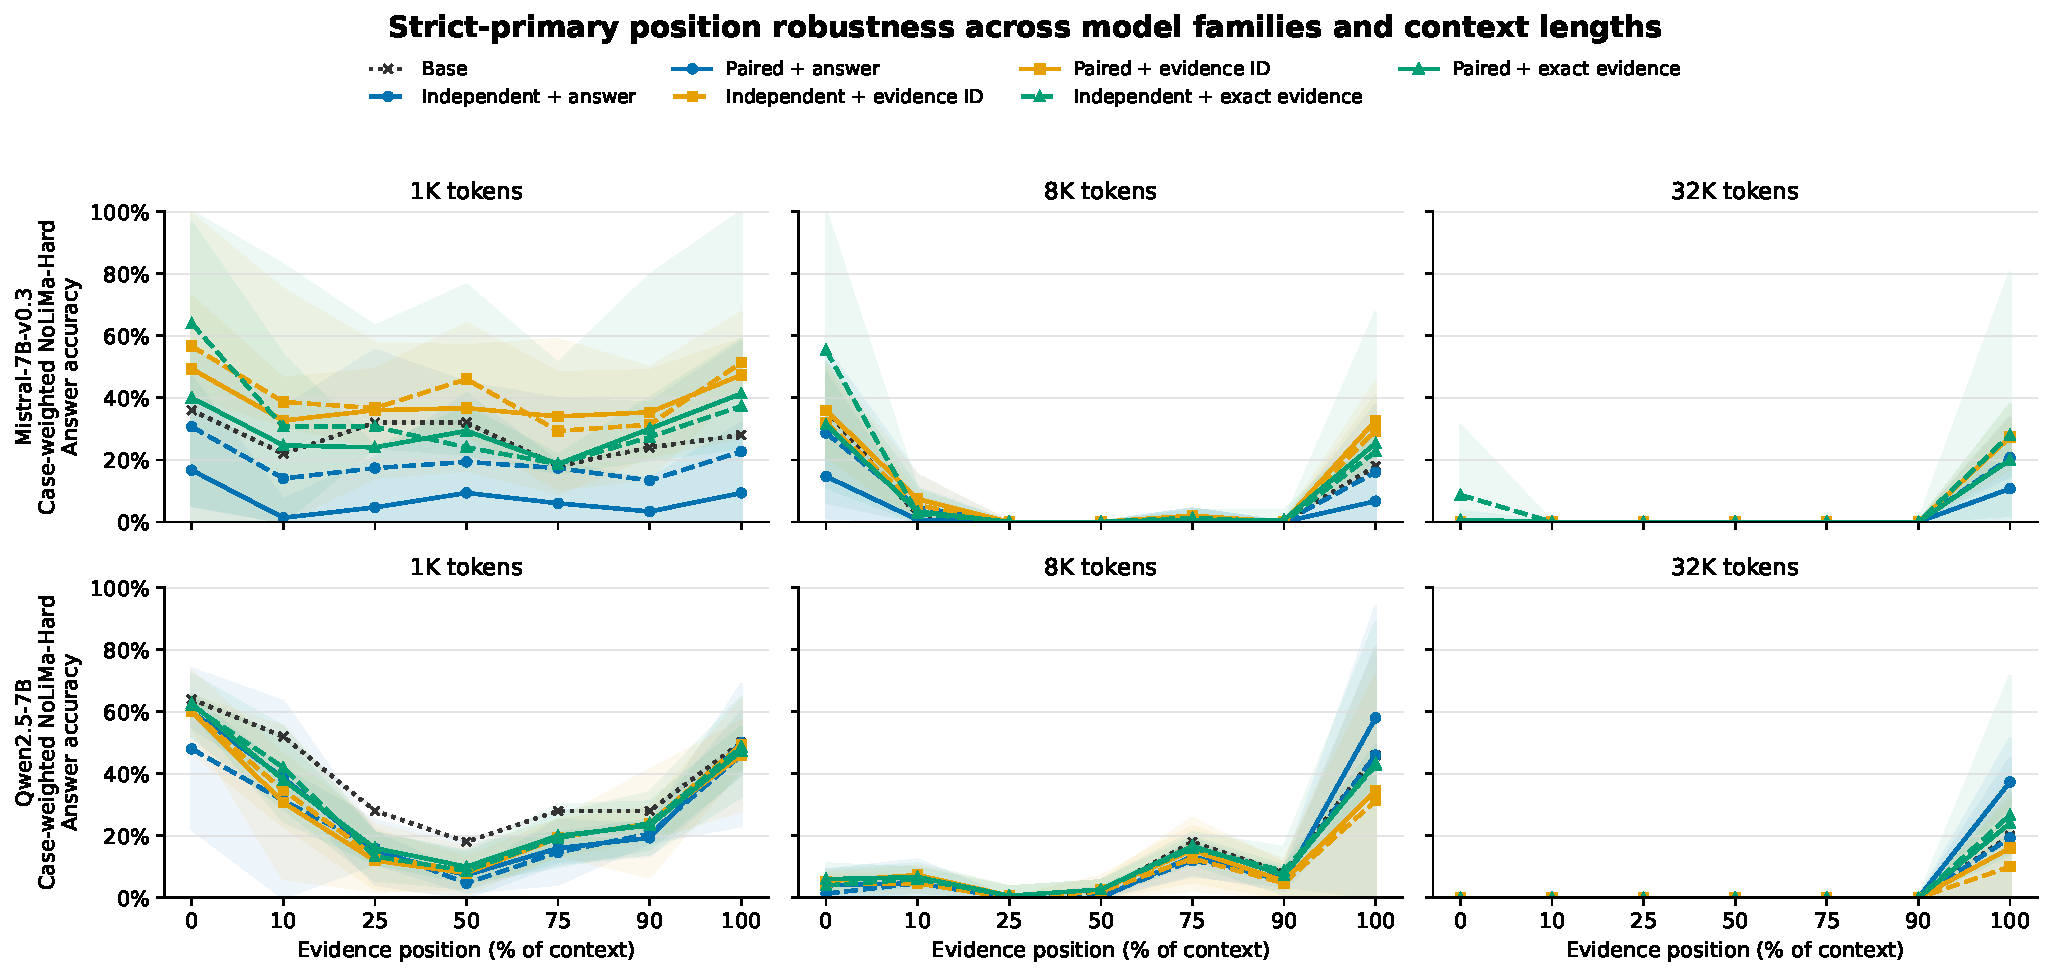
\includegraphics[width=\textwidth]{figures/factorial_position_curves.pdf}%
}{\fbox{\parbox{0.94\textwidth}{\centering\pending{复制已审计的析因位置图}}}}
\caption{主严格块完备 NoLiMa-Hard 七个证据位置上的答案准确率，在三个任务层的 2/6/2 底层语义案例上案例加权。行为模型家族、列为上下文长度。颜色表示监督粒度，实线对虚线表示配对对独立构造。带为独立训练种子上的 95\% Student-$t$ 区间，仅为显示裁剪；固定基座无种子区间，精确值见配套 CSV。}
\label{fig:position}
\end{figure*}

\subsection{自然多文档迁移}

没有严格处理在 Qwen 上超过其家族基座（表~\ref{tab:longbench}；汇总 token-F1 39.0--42.8，基座 43.7），且 Qwen 析因对比与零不可区分（如证据 ID 减仅答案 $-1.4$ $[-7.9,+5.2]$）。Mistral 呈现相反的粒度模式：两个证据 ID 单元迁移超过基座（38.3 与 36.5 对 32.7），而两个精确引文单元低于基座约十个点（22.6 与 22.1），精确证据减仅答案对比为 $-6.8$ $[-15.5,+2.0]$。描述性地，Mistral 减 Qwen 家族差对证据 ID 监督为 $+9.6$ 个百分点、对精确引文为 $-7.8$ 个百分点。由于 LongBench 在此不标注可移动的黄金证据，这些分数仅确立自然迁移：面向可验证性的监督并不一致地帮助自然任务且可能有害，其符号依赖监督粒度与家族。

\begin{table*}[t]
\centering
\small
\caption{主严格块完备 LongBench 多文档 QA token-F1。处理值为独立训练种子均值，基座固定。分数使用官方英文 QA 对参考答案的最大 F1；三个任务各含 200 个问题。}
\label{tab:longbench}
\begin{tabular}{lllrrrr}
\toprule
模型 & 配对 & 监督 & HotpotQA & 2WikiMQA & MuSiQue & 汇总 \\
\midrule
\GeneratedLongBenchRows
\bottomrule
\end{tabular}
\end{table*}

\begin{table*}[t]
\centering
\scriptsize
\setlength{\tabcolsep}{3pt}
\caption{关键严格块完备析因对比（百分点），格式为种子级均值 [95\% Student-$t$ 区间]。$\Delta$最差为正更好，$\Delta$差距为正更差；LongBench $\Delta$F1 为正更好。这些对比先于实际子集修正而定义；完整每种子对比、种子内配对自助区间与 Holm 校正检验包含在发布的分析文件中。}
\label{tab:factorial-contrasts}
\resizebox{\textwidth}{!}{\begin{tabular}{llrrrrr}
\toprule
模型 & 对比 & 规则$\Delta$最差 & 规则$\Delta$差距 & NoLiMa$\Delta$最差 & NoLiMa$\Delta$差距 & LongBench$\Delta$F1 \\
\midrule
\GeneratedFactorialContrastRows
\bottomrule
\end{tabular}}
\end{table*}

\subsection{机制与能力保持}

探索性 Qwen 代表分离了三种原本混淆的失败模式。Base 与全部四个角处理的 oracle-short 性能接近天花板，因此从孤立黄金段落生成答案不是主导瓶颈。精确证据处理将 locate-only 引文从 6.0\%（基座）提升到 34.7--35.8\%，但该增益未带入自由答案准确率或干扰下的 oracle-long 证据使用。配对仅答案监督是唯一提升 oracle-long 准确率（0.7\% 到 2.0\%）的 Qwen 角，其自由答案分数仍不超过基座，与``更好利用已暴露证据但定位未解决''一致。这些代表种子诊断不是多种子处理估计；表~\ref{tab:mechanism} 报告聚类区间。回归检查中（表~\ref{tab:regression}），Qwen MMLU 重分析在正确性与 JSON 闭包分离后对每个处理都通过冻结的两点非劣性边界。IFEval 无 Holm 显著处理差异，但其严格提示区间无一建立同样的非劣性保证。Mistral 回归检查映照其析因不稳定性：配对仅答案训练丢失约二十个 MMLU 点（34.3\% 对基座 54.2\%）与一半 IFEval 严格提示准确率（21.3\% 对 43.1\%），正是规则与 NoLiMa 套件上崩溃的同一单元；其余 Mistral 单元通过 MMLU 非劣性，独立精确引文训练是唯一通过 IFEval 非劣性的 Mistral 单元。因此我们将该单元行为视为单一低预算配置的优化不稳定，而非家族级能力代价。

\begin{table*}[t]
\centering
\small
\caption{代表种子短上下文回归检查。MMLU 为全量测试格式稳健选项准确率，IFEval 为官方严格提示准确率。非劣性（NI）仅当处理减基座的配对 95\% 区间完全高于冻结的 $-2$ pp 边界时通过。JSON 有效性单独审计，且不是 MMLU 正确性的前提。}
\label{tab:regression}
\begin{tabular}{lllrrrr}
\toprule
模型 & 配对 & 监督 & MMLU & MMLU NI & IFEval & IFEval NI \\
\midrule
\GeneratedRegressionRows
\bottomrule
\end{tabular}
\end{table*}

\begin{table*}[t]
\centering
\small
\caption{代表种子 NoLiMa 机制分解。Locate-only 请求引文；oracle-long 将黄金证据移至相同长干扰上下文之后的带标签块；oracle-short 移除干扰。数值在 10 个语义案例上聚类。}
\label{tab:mechanism}
\resizebox{\textwidth}{!}{\begin{tabular}{lllrrrr}
\toprule
模型 & 配对 & 监督 & 自由答案 & 定位引文 & Oracle 长 & Oracle 短 \\
\midrule
\GeneratedMechanismRows
\bottomrule
\end{tabular}}
\end{table*}

\subsection{描述性失败分类}

两个历史试点后 fixed-100 Qwen NoLiMa 目录在定性失败形状上一致。在约十分之九的适用运行内组中，答案在七个位置间发生变化；边缘成功/中部失败组约为反向模式的四倍。无效 JSON 与输出上限命中保持在一成以下，因此格式失败无法解释低语义答案准确率。在匹配的基座--处理比较中，两个种子里基座专属成功都多于处理专属成功，与部分剂量处理优势的缺失一致。严格目录（18 个已审计套件、两家族）在失败层面确认了修复：规则套件上，答案在 11.7\%（Qwen）与 20.6\%（Mistral）的适用组中跨七位置变化，远低于历史 fixed-100 约十分之九的比率；Qwen 上边缘成功/中部失败与中部成功/边缘失败组几乎等率（9.5\% 对 10.6\%），与压平的位置曲线一致，而 Mistral 保留边缘方向不对称（18.5\% 对 9.3\%）。格式无法解释残余错误：无效 JSON 与输出上限命中在每个严格套件中保持不超过 3.1\%。NoLiMa 上失败形状回退：答案在 90.2\%（Qwen）与 69.2\%（Mistral）的适用组中跨位置变化，两家族中边缘成功/中部失败组都以约 3.6 比 1 超过反向（44.6\% 对 12.4\%、38.2\% 对 10.6\%）；匹配比较在 Qwen 上倾向基座（基座专属成功 5.1\% 对处理专属 1.8\%），Mistral 上平衡（4.6\% 对 5.2\%）。标识符指纹化的逐案例记录复现这些聚合比率且不含基准文本；我们用其说明而非选择处理。三种分母类型保持分离，这些案例仅用于说明聚合结果，不用于选择处理或追加事后显著性声明。

\section{讨论}

析因设计分离了三个常被混淆的结论。第一，平坦的分布内位置曲线可与差的语义或自然迁移共存。第二，仅答案正确性不能确立可验证的证据使用。第三，均衡位置直方图未必等价于跨位置展示同一底层事实。严格结果强化了全部三点。受控套件修复真实存在但呈因子化的家族依赖：Qwen 上监督粒度区分单元而位置构造不区分；Mistral 上两因素交互强到配对仅答案训练是最差单元、配对精确引文训练是最佳单元。修复也是分布特定的：NoLiMa 上每个 Qwen 单元仍在基座之下，仅 Mistral 证据 ID 单元勉强超过其基座，因此压平受控曲线的同一单元使语义检索不变或退化。监督粒度跨场景权衡而非单调排序：标识符监督在 NoLiMa 上最温和、是 Mistral LongBench 上唯一超过基座者，而精确引文最大化受控套件引文保真度却在 Mistral LongBench 上损失约十个点。

本实验设计为支持有信息量的阴性结果。若全部六个严格 block-96 处理收敛到同一分布外分数，可支持的结论是：单次低预算监督修复在可得分辨率下对这些因素不敏感。若规则准确率改进而 NoLiMa 与 LongBench 不改进，结论是分布特定的记忆或模板适应，而非稳健的上下文利用。

\section{局限}

本研究使用两个约 7B 的模型家族，无法确立标度律。QLoRA 与全参数训练相比，可能与模型家族及位置编码产生不同交互。严格回调在 2,000 步余弦调度的 60 步预热加 36 步处、即第 96 步停止；这是低预算单次适配器机制，而非优化的全收敛配方。因此我们的归因关于该固定机制下哪些因素有帮助，而非更长或全参数训练能否消除该失败。严格修正仅在 Qwen NoLiMa 与部分 LongBench 输出已存在之后设计。其选择规则确定、与分数无关、且应用于全部六个单元与全部三个种子，但 Qwen 修正仍是事后的；仅 Mistral 前瞻性地检验了修正设计。我们保留原始 fixed-100 产物及其未通过的实际子集门禁，使该局限可独立审计。NoLiMa-Hard 门禁仅含 10 个底层语义案例在书本、长度与放置上重复；推断必须尊重该分组，主张不能把 1,050 条提示当作独立语义问题。LongBench 提供自然上下文，但所选任务中没有受控证据重置或精确证据标签。每个模型家族的确定性基座生成跨处理种子复用，而非作为独立的模型训练复现呈现；因此种子级处理区间量化的是固定基座周围的适配器/数据种子变异，而非基座预训练或模型选择上的不确定性。相应地，种子级区间必然较宽，跨家族差异作为描述性交互而非精确总体估计处理。最后，精确引文是可验证性代理，不是忠实推理的完整度量。

\section{伦理、许可与可复现性}

NoLiMa 数据在 Adobe Research License 下用于非商业研究，以来源指针与生成哈希分发而非再许可。LongBench 仓库在 Massachusetts Institute of Technology (MIT) License 下发布，各组成数据集保留其原始条款。合成数据包含生成的事实而非个人信息。公开失败目录以单向指纹替代基准文本与原始标识符。我们不发布任何模型服务凭据、机器密码或私有路径。

完整的已审计证据树保留每个结果行及其模型条件、样本与位置等价组、目标、原始生成、解析 JSON、适用度量、结束原因与输出 token 数。公开发布排除原始基准与生成 JSONL，而非静默再许可基准文本；它提供固定的重建脚本与哈希、许可安全的逐样本失败记录、模型版本与文件哈希、数据清单、环境与 GPU 元数据、逐步训练轨迹、全部自助法索引、分析 CSV/JSON、以及带表格替代与替代文本的矢量/栅格图。

全部训练与生成工作负载在一台 32 GB RTX 5090 级实例上顺序执行，而非隐藏在多实例并行之后。已审计账目记录 188 个顺序 GPU 事件、共 118.5 有效 GPU 小时（评测 115.9、训练 2.6）与 329.42 人民币（CNY）的租赁成本下界；严格队列跨越 2026-08-29 至 2026-09-04 墙钟，包含一次操作者发起的关机与一次无损的审计门禁恢复。我们报告实测硬件与墙钟时间以便算力比较，但不估计碳排放，因为云厂商不披露本次租赁的机器电力归因、数据中心位置或电力使用效率（PUE）。

\section{结论}

我们提出了一套匹配析因框架，将长上下文位置稳健性归因于显式跨位置配对与监督粒度，一套位置等价评测协议、互补的受控与自然分布偏移测试，以及带审计谱系的可复现性包。在跨两个模型家族复制的已审计严格块完备协议下，单次 96 步训练大幅修复了受控最差位置准确率，但有效因素随家族而异，且没有任何处理把该修复带到无字面重叠的语义检索或自然多文档问答；监督粒度甚至在后者上跨家族反号。配对假设的强形式——跨位置看到同一事实优于匹配的独立直方图——仅在一个家族上作为与可验证监督的交互获得支持。我们发布完整审计轨迹、适配器与分析代码，使这些低预算位置稳健性训练的边界条件可被验证与扩展。

\appendix

\section{冻结训练配置}

全部严格主单元使用表~\ref{tab:training-config} 所示的相同实现与超参数。一次运行只从其自身最新检查点恢复；已审计的第 96 步检查点绝不重训。模型权重从固定版本的本地快照加载，分词数据必须在与 tokenizer 及对话模板指纹匹配之后才能开始 CUDA 工作。历史第 100 步产物保留在独立根目录下，无法满足主完成门禁。

\begin{table}[h]
\centering
\small
\caption{每个严格主处理的冻结 QLoRA 配置。}
\label{tab:training-config}
\begin{tabularx}{\linewidth}{@{}lX@{}}
\toprule
项目 & 取值 \\
\midrule
量化 & 4-bit NF4，双重量化，BF16 计算 \\
LoRA & 秩 16，$\alpha=32$，dropout 0.05，全部线性层 \\
目标 & 仅完成部分交叉熵，无打包 \\
最大序列长度 & 8,320 token \\
批处理 & 每设备 1 序列，累计 1 \\
优化器 & paged AdamW 8-bit \\
学习率调度 & 峰值 $2\times10^{-4}$；2,000 步余弦 \\
预热与停止 & 60 步预热（调度 3\%）；恰在第 96 步回调 \\
精度/运行时 & BF16、TF32、梯度检查点、缩放点积注意力（SDPA） \\
种子 ID & 20260825、20260826、20260827；Qwen 重跑为事后修正，Mistral 前瞻 \\
\bottomrule
\end{tabularx}
\end{table}

\section{评测与解码清单}

表~\ref{tab:evaluation-config} 记录冻结的推理窗口与解码上限。每个渲染提示加其输出上限必须 fit 所列窗口；窗口值不呈现为实际提示长度。全部套件使用贪心解码（温度 0）与固定运行时种子；批大小与 vLLM 引擎设置按运行记录并在每套件内保持恒定。受控规则、NoLiMa、LongBench 与 MMLU 生成请求模式约束 JSON。对前三个套件，格式有效性是结构化任务诊断的一部分。对 MMLU，正确性独立于 JSON 闭包从选项字母重评分，同时有效性与截断单独报告。IFEval 刻意不加约束，因为官方指令常要求精确的自在格式；其原始文本由固定的官方验证器评分。

\begin{table}[h]
\centering
\small
\caption{每模型条件的评测清单。计数不含自助复制。}
\label{tab:evaluation-config}
\begin{tabular}{lrrrl}
\toprule
套件 & 行数 & 窗口 & 最大输出 & 主单元 \\
\midrule
匹配规则 & 4,200 & 32,768 & 176 & 位置等价组 \\
NoLiMa-Hard & 1,050 & 32,768 & 176 & 语义案例/组 \\
LongBench QA & 600 & 32,768 & 96 & 基准问题 \\
NoLiMa 诊断 & 1,350 & 32,768 & 176 & 语义案例 \\
MMLU & 14,042 & 2,048 & 32 & 测试题 \\
IFEval & 541 & 4,096 & 1,024 & 提示/指令 \\
\bottomrule
\end{tabular}
\end{table}

\section{产物与主张审计}

发布区分原始生成、种子内配对自助分析、种子级摘要与论文面向数字。原始输出是带不可变数据与适配器哈希的可恢复 JSON Lines (JSONL) 文件。每个种子内分析保存其 5,000 个重采样索引。种子级聚合显式接受探索性、修正性与验证性标注；探索性运行排除在主摘要之外，而每个纳入的模型家族必须至少有两个独立训练的合格种子。最后，生成的 TeX 表记录全部种子级输入的 SHA-256 值；投稿审计拒绝未解决的占位符、缺失的图或引用、机密与绝对机器路径。作者元数据仍是唯一无法自主完成的非实验项。

\bibliographystyle{plainnat}
\bibliography{references}

\end{document}
